\begin{document}

La protocol proposat en \cite{busom} es basa en un sistema agregatiu, on la subestació només sabrà el valor en conjunt d'un barri de comptadors agregats, és a dir, el sumatori de cadascuna de les seves lectures. En aquesta proposta, es vol utilitzar una clau pública per tal d'encriptar les dades i, gràcies a la propietat homomòrfica d'ElGamal, rebre només el resultat en conjunt. Per tal de complir aquest objectiu, hi ha una fase de configuració de claus i una altra, que tractarà l'enviament xifrat dels missatges, tal i com es mostra en la \textit{Figura \ref{fig:busom}}.
\begin{figure}
	\centering
	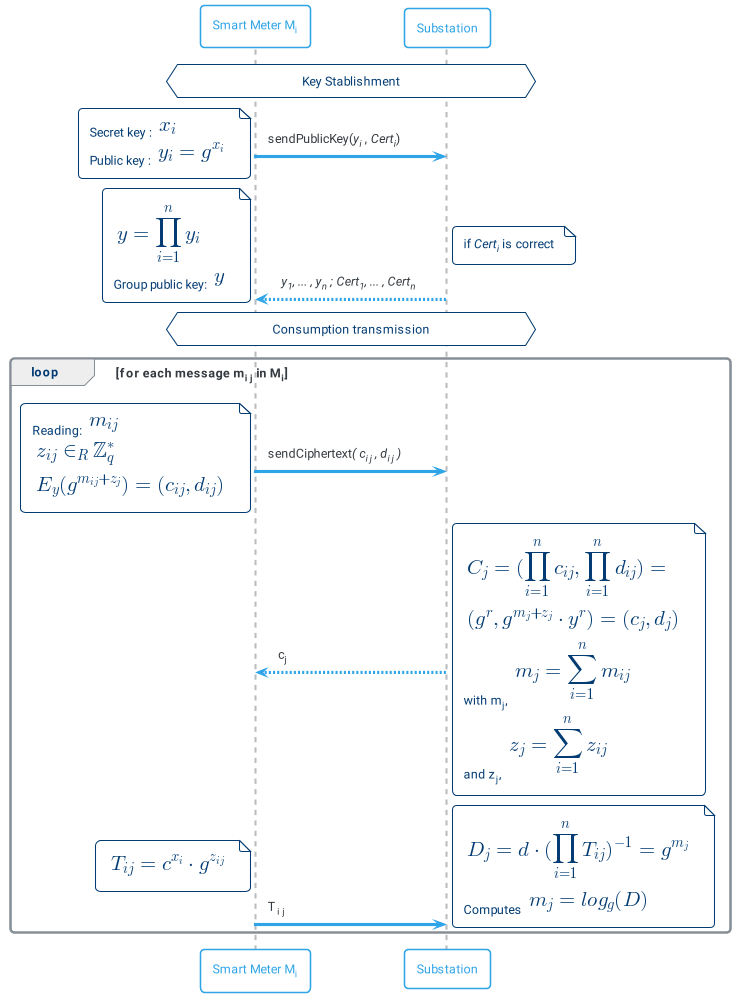
\includegraphics[width=14cm]{umls/busom.png}
	\caption{Diagrama de seqüència del protocol Busom}
	\label{fig:busom}
\end{figure}

\subsubsection{Procediment}
\myparagraph{Configuració del sistema}
Al ser un protocol de tipus agregatiu utilitzant el sistema criptogràfic ElGamal amb la propietat homomòrfica en la multiplicació, la configuració del sistema serà el següent:
\begin{itemize}
	\item Dos primers $p$ i $q$ sent $p = 2q+1$.
	\item Un generador $g \in \mathbb{Z}_p^*$ d'ordre $q$.
	\item Un sistema de certificats digitals perquè la subestació reconegui els comptadors intel·ligents del seu barri.
\end{itemize}
\myparagraph{Establiment de clau pública Diffie-Hellman}
Per tal d'escollir la clau pública, es proposa usar el sistema d'intercanvi de claus Diffie-Hellman. \cite{busom} posa en pràctica aquest intercanvi de claus per tal de xifrar els consums d'electricitats dels comptadors a la subestació. Cada comptador té la seva clau secreta\footnote{La clau secreta és creada de manera aleatòria.} $x_i \in \mathbb{Z_q^*} $ i fan públic $y_i = g^x$ juntament amb una prova zero-knowledge\footnote{Protocol que estableix un mètode per comprovar quelcom sense haver de revelar la veracitat de la declaració. En aquest cas, s'ha de comprovar que el comptador forma part del conjunt o barri.} sobre $log_g(y_i)$, per tal que la subestació ho verifiqui i faci calcular $y = \prod_{i=1}^{n} y_i$ a les subestacions.
\myparagraph{Transmissió del consum}
No obstant s'ha aconseguit una clau per tal de xifrar els consums, encara no s'ha aconseguit privacitat en les llars, ja que la subestació sabria el valor de les lectures. Per tal de fer-ho, s'obtindrà l'avantatge de la propietat homomòrfica d'ElGamal per tal de protegir les dades. Per tal d'entendre bé aquest procés, relaxarem el problema de manera que només es fa una iteració. El nombre que representa la iteració $j$, en aquest cas serà $j = 1$.
\begin{enumerate}
	\item La subestació sol·licitarà als comptadors les lectures de l'electricitat. En el cas real, la subestació ho demanaria de manera periòdica i cada vegada $j$ incrementaria.
	\item Cada comptador generarà un soroll aleatori $z_i \in {\mathbb{Z}_{q}^*}_R$ i enviarà a la subestació la següent computació: 
	\[C_i = E_y(g^{(m_i + z_i)}) = (c_i, d_i) = (g^r_i, m_i y^r_i)\]
	\item La subestació agrega tots els xifrats de manera que:
	
	\[C = (\prod_{i=1}^{n} c_i, \ \prod_{i=1}^{n} d_i) = (g^r, \ y^r \cdot \prod_{i=1}^{n} m_i) = (c, d)\]
	
	i envia $C$ a tots els comptadors del seu barri.\label{en:busom-s1}
	\item Cada comptador, al rebre $C$, computa:
	\[T_i = c^{x_i} g^{z_i}\]
	i envia el seu resultat a la subestació. Després d'això, el comptador ja no necessitarà $z_i$ i podrà esborrar-lo de la memòria.\label{en:busom-m1}
	\item Un cop la subestació ha rebut tots els $T_i$ de cada comptador, calcula:
	\[D = d \cdot (\prod_{i=1}^{n} T_i)^{-1}, \qquad \prod_{i=1}^{n} T_i = (g^{r})^x \cdot g^z = y^r \cdot g^z\]
	\item D'aquesta manera, la subestació només haurà de calcular:
	\[m = log_g D = \sum_{i=1}^{n} m_i\]
	Al necessitar realitzar el logaritme discret, es requereix que les lectures siguin petites per tal de no elevar el cost computacional.
\end{enumerate}
% cost lineal O(n)
\subsubsection{Problema amb la privacitat de les lectures}
En \cite{repair-busom} s'explica com una subestació corrupta, sense necessitat de la col·laboració de cap comptador intel·ligent corrupte, pot obtenir la lectura exacta del consum d'un comptador intel·ligent dirigit a una ronda determinada del protocol.
\\
\\
La subestació, per tal d'aconseguir aquesta lectura, s'ha de desviar del protocol en una ronda determinada, en la qual no obtindrà cap informació sobre les lectures enviades pels comptadors. No obstant això la informació en el missatge xifrat serà obtingut en la següent ronda. Per tal de aconseguir la lectura sobre un comptador en la fase de transmissió de les dades, es realitza:
\begin{enumerate}
	\item Primera ronda.
	\begin{enumerate}
		\item En lloc d'enviar $c \in C$ tal i com es diu en el pas \ref{en:busom-s1}, la subestació envia $\hat{c}$ generant de manera aleatòria un valor $v$:
		\[\hat{c} = g^v \quad t.q \quad v \in {\mathbb{Z}_{q}}_R\]
		\item Els comptadors, realitzaran de forma normal l'operació del pas \ref{en:busom-m1}, retornant com a resultat:
		\[\hat{T}_i = (\hat{c})^{x_i} \cdot g^{z_i} = (g^v)^{x_i} \cdot g^{z_i} = y_i^v \cdot g^{z_i}\]
		\item Gràcies a que el valor $y_i$ de cada comptador és la seva clau pública, la subestació pot saber $g^{z_i}$ realitzant:
		\[g^{z_i} = \hat{T}_i \cdot (y_i^v)^{-1}\]
		D'aquesta manera, sabent que $E_y(g^{m_i + z_i}) = (c_i, d_i) = (g^{r_i}, \; g^{m_i + z_i}) \cdot y^{r_i}$, la subestació pot saber $E_y(g^{m_i})$:
		\[E_y(g^{m_i}) = (c_i, d_i \cdot (g^{z_i})^{-1}) = (g^{r_i}, \; g^{m_i} \cdot y^{r_i}) = (c', d')\]
	\end{enumerate}
	La operació que realitza la subestació per tal de saber $E_y(g^{m_i})$ es pot realitzar sobre tots els comptadors en la mateixa ronda, per tal de saber la lectura de tots.
	\item Segona ronda.
	\begin{enumerate}
		\item La subestació en aquest pas, després d'agregar de forma usual els xifrats dels comptadors obtenint així $C = (c, d)$, computa:
		\[(c'', d'') = (c \; \cdot \; (c')^{m_{max}}, \; d \; \cdot (d')^{m_{\textrm{max}}})\]
		sent:
		\begin{itemize}
			\item $c'$ el primer component de $E_y(g^{m_i}) = (c', d') = (g^{r_i}, d')$.
			\item $c$ el primer component de l'agregació de xifrats en la segona ronda $C = (c,d)$.
			\item $m_{\textrm{max}}$ sent una fita superior de la suma de lectures dels comptadors en una ronda.
		\end{itemize}
		Sabent això, es pot veure que, de la mateixa manera $E_y(g^m+z) = (c, d) = (g^r, g^{m+z} \cdot y^r)$:
		\begin{align*}
		E_y(g^{m + z + m_i'\cdot m_{\textrm{max}}}) &= (g^{r + r_i \cdot m_{\textrm{max}}}, \;\; g^{m + z + m_i' \cdot m_{\textrm{max}}} \; \cdot \; y^{r + r_i \cdot m_{\textrm{max}}}) \\
		&= ( g^r \; \cdot g^{r_i \cdot m_{\textrm{max}}} , \;\; g^{m + z} \cdot y^r \cdot g^{m_i' \cdot m_{\textrm{max}}} \cdot y^{r_i \cdot m_{\textrm{max}}} )\\
		&= (g^r \cdot (g^{r_i})^{m_{\textrm{max}}}, \;\; g^{m + z} \cdot y^r \cdot (g^{m_i'} \cdot y^{r_i})^{m_{\textrm{max}}} )\\
		&=(c \cdot (c')^{m_{\textrm{max}}}, \;\; d \cdot (d')^{m_{\textrm{max}}})\\
		&=(c'', d'')
		\end{align*}
		Així doncs, la subestació envia $c''$ a tots els comptadors.
		\item Cada comptador computa de manera innocent i envia a la subestació:
		\[T_i'' = (c'')^{x_i} \cdot g^{z_i}\]
		\item D'aquesta manera, la subestació troba:
		\[D'' = d'' (\prod T_i'')^{-1} = g^{m + m_i' \cdot m_{\textrm{max}}}\]
		Realitzant el logaritme discret de $D''$ en base $g$ trobem $m + m_i \cdot m_{\textrm{max}}$, que és fàcil de descompondre, ja que $m_{\textrm{max}} > m$. D'aquesta manera, es troba $m_i$ que correspon a la lectura del comptador $i$ de la ronda anterior.\\
		El creixement en complexitat temporal per resoldre el logaritme discret és incrementat aproximadament per un factor de $\sqrt{m_{\textrm{max}}} $, que depèn el nombre de comptadors intel·ligents associats al barri.
	\end{enumerate}
\end{enumerate}
Aquest atac es pot realitzar de manera distribuïda en tots els comptadors intel·ligents, és a dir, d'una ronda en específic es pot agafar les lectures de tots els comptadors. No obstant això, el preu que es paga per realitzar-ho és perdre la lectura dels comptadors de la ronda següent.
\myparagraph{Sol·lució proposada}
\begin{figure}[H]
	\centering
	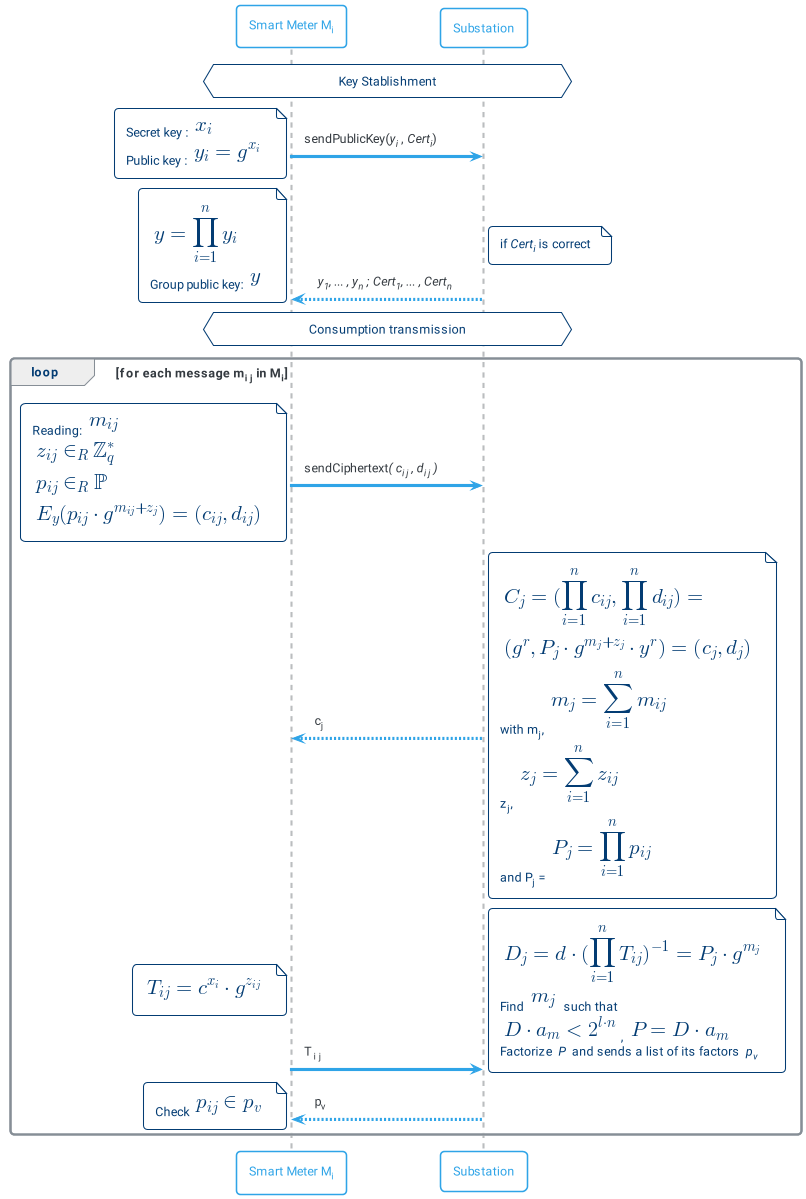
\includegraphics[width=13cm]{umls/garra.png}
	\caption{Diagrama de seqüència de la sol·lució proposada en el problema de la privacitat de Busom}
	\label{fig:garra}
\end{figure}
Per tal de resoldre el problema amb la privacitat recentment esmentat, en \cite{repair-busom} es proposa una modificació del protocol per a que al final de cada ronda, la subestació hagi d'estar forçada a enviar als comptadors una prova que s'ha format el protocol de manera correcta. El diagrama de seqüència d'aquest nou sistema es troba la \cref{fig:garra}. En cas de no superar la prova, els comptadors requeriran tornar a realitzar una nova configuració de claus. En el procediment s'afegeix:
\begin{enumerate}
	\item En la \textit{configuració del sistema}, s'afegirà del original:
	\begin{itemize}
		\item La constant $l \ge 16 $ que satisfà \[l \cdot n \le \lfloor log_2 \; p \rfloor - 64\]
		\item \textit{Precomputació de taula de primers}. Cada comptador $M_i$ guarda una taula amb tots els enters primers $p_i$, de llargada en bits com a màxim $l$, $\lceil log_2 \, p_i \rceil \le l$, que pertanyen a $\mathbb{Z_q^*}$ i estan generats per g.
		\item \textit{Vector de precomputació}. La subestació computa i guarda un vector $a = (a_0, \dots, a_{m_{\textrm{max}}})$ tal que \[a_i = (g^i)^{-1}, \quad i \in \{0, \cdots, m_{\textrm{max}}\}\] sent $m_{\textrm{max}}$ una fita superior de la suma de totes les lectures del comptadors del sistema agregat.
	\end{itemize}
	\item L'\textit{establiment de claus} no varia de la versió original \cite{busom}, ja que no hi ha incidències de seguretat en aquesta fase del sistema.
	\item Per tal d'explicar els canvis en la \textit{transmissió del consum}, s'ha preferit explicar tot el procès de comunicació.
	\begin{enumerate}
		\item La subestació demana a tots els comptadors intel·ligents que pertanyen al seu barri les seves lectures mitjançant un missatge de sol·licitud.
		\item Cada comptador $M_i$ genera un aleatori $z_i \in_R \mathbb{Z_q^*}$ i agafa un primer aleatori $p_i < 2^l$ de la seva memòria interna en la taula de precomputacióz. Llavors, el missatge xifrat està compost per la lectura en el temps actual $m_i$, el generador $g$, el valor aleatori $z_i$ i el nou primer aleatori $p_i$ de tal manera:
		\[E_y(p_i \cdot g^{m_i + z_i}) = (c_i, d_i) = (g^r, p_i \cdot g^{m_i + z_i} \cdot y^{r_i})\]
		\item La subestació agregarà tots els missatges xifrats rebuts
		\[(c, d) = \Big( \prod c_i, \; \prod d_i \Big) = (g^r,\; P \cdot g^{m + z} \cdot y^r)\]
		sent $m = \sum m_i$, $z = \sum z_i$ i $P = \prod p_i$ i enviarà el component $c$ a cada comptador.
		\item Cada comptador $M_i$ realitzarà $T_i = c^{x_i} \cdot g^{z_i}$ i envia el resultat a la subestació. En aquest punt de comunicació, $M_i$ eliminarà $z_i$ de la seva memòria.
		\item Un cop la subestació rep tots els $T_i$, computarà:
		\[D = d \cdot \Big( T_i \Big)^{-1} = P \cdot g^m\]
		Com que $P < 2^{l \cdot n}$, ja que cada $p_i$ té, com a màxim, d'ordre de $l$ bits , la subestació podrà determinar $m$ mitjançant
		\[D \cdot a_m  < 2^{l \cdot n}\]
		A més a més, com que $D \cdot a_m = P \cdot g^m \cdot a_m = P \cdot g^m \cdot (g^m)^{-1} = P$, la subestació pot factoritzar $P$ i enviar els primers resultants en una llista ordenada $p_v$ a cada comptador.
		\item Cada comptador comprova que la llargada de $p_v$ és $|p_v| = n$ i que $p_i \in p_v$. En cas que la comprovació d'algun comptador fallés, aquest hauria de demanar tornar a la fase d'establiment de claus i totes les claus publiques haurien de ser renovades. D'aquesta manera, els comptadors saben que la subestació no els ha estat enganyant per tal d'atacar la seva privacitat
		
	\end{enumerate}
\end{enumerate}

\end{document}
